% These are the lecture notes for my CSCI360 course SPRING 2017
% at John Jay College of Criminal Justice. They are based largely on
% Schneier's Applied Cryptography.

% Feel free to edit these slides and use them for your own courses.
% HOWEVER DO NOT REMOVE THESE LINES!
% Email me at: awood [at] jjay.cuny.edu
% or at: awood [at] gradcenter.cuny.edu


\documentclass{beamer}

\usepackage{tikz}
\usetikzlibrary{calc}

\usepackage{forest}
\usepackage{verbatim}
\usepackage{color}
\usepackage{amsmath}
\usepackage{graphicx}
\usepackage{caption}



\setbeamertemplate{footline}[frame number]
\setbeamertemplate{navigation symbols}{} 

\newtheorem{thm}{Theorem}[section]
\newtheorem{lem}{Lemma}
\newtheorem{cl}{Claim}
\newtheorem{cor}{Corollary}[section]
\newtheorem{conj}{Conjecture}
\newtheorem{quest}{Question}
\newtheorem{defn}{Definition}[section]
\newtheorem{obs}{Observation}[section]
\newtheorem{exam}{Example}

\newcommand{\im}{\operatorname{im}}
\newcommand{\id}{\operatorname{id}}
\newcommand{\interior}{\operatorname{int}}
\newcommand{\bdry}{\operatorname{bdry}}
\newcommand{\<}{\langle}
\renewcommand{\>}{\rangle}
\newcommand{\Gab}{(G_\phi)^{ab}} 
\newcommand{\phibar}{\bar{\phi}}
\newcommand{\Z}{\mathbb{Z}}
\newcommand{\N}{\mathbb{N}}
\newcommand{\Q}{\mathbb{Q}}
\newcommand{\R}{\mathbb{R}}
\newcommand{\C}{\mathbb{C}}
\newcommand{\A}{\mathcal{A}}
\newcommand{\OO}{\mathcal{O}}
\newcommand{\UU}{\mathcal{U}}
\newcommand{\power}{2^{\{P_1, \cdots , P_n\}}}
\newcommand{\bp}{\begin{problem}}
\newcommand{\ep}{\end{problem}}
\newcommand{\ba}{\begin{answer}}
\newcommand{\ea}{\end{answer}}
\newcommand{\ds}{\displaystyle}
\newcommand{\ben}{\renewcommand{\theenumi}{\alph{enumi}}
\renewcommand{\labelenumi}{(\theenumi)}\begin{enumerate}}
\newcommand{\een}{\end{enumerate}}
\newcommand{\Hess}{\operatorname{Hessian}}
\newcommand{\Aut}{\mathrm{Aut}}
\newcommand{\Inn}{\mathrm{Inn}}
\newcommand{\Out}{\mathrm{Out}}
\newcommand{\End}{\mathrm{End}}


\mode<presentation>
{
%  \usetheme{default}
  \setbeamercovered{invisible}
}


\usepackage[english]{babel}
\usepackage[latin1]{inputenc}
\usepackage{times}
\usepackage[T1]{fontenc}
\usepackage{stmaryrd}

%\usetheme{default}
%\usetheme{AnnArbor}
%\usetheme{Antibes}
%\usetheme{Bergen}
%\usetheme{Berkeley}
%\usetheme{Berlin}
%\usetheme{Boadilla}
%\usetheme{CambridgeUS}
%\usetheme{Copenhagen}
%\usetheme{Darmstadt}
%\usetheme{Dresden}
%\usetheme{Frankfurt}
%\usetheme{Goettingen}
%\usetheme{Hannover}
%\usetheme{Ilmenau}
%\usetheme{JuanLesPins}
%\usetheme{Luebeck}
%\usetheme{Madrid}
%\usetheme{Malmoe}
%\usetheme{Marburg}
%\usetheme{Montpellier}
%\usetheme{PaloAlto}
%\usetheme{Pittsburgh}
%\usetheme{Rochester}
\usetheme{Singapore}
%\usetheme{Szeged}
%\usetheme{Warsaw}

%\usecolortheme{default}
%\usecolortheme{albatross}
\usecolortheme{beaver}
%\usecolortheme{beetle}
%\usecolortheme{crane}
%\usecolortheme{dolphin}
%\usecolortheme{dove} % grey, white, yellow
%\usecolortheme{fly} %grey, yellow
%\usecolortheme{lily} %white, yellow, blue
%\usecolortheme{orchid}
%\usecolortheme{rose}
%\usecolortheme{seagull}
%\usecolortheme{seahorse}
%\usecolortheme{whale}
%\usecolortheme{wolverine}

% Title page

\title[DES]{Implementing DES}

\subtitle{Based on \emph{Applied Cryptography} by Schneier, Chapter 12}

\author
{Lecture notes of Alexander Wood \\ \scriptsize \href{mailto:awood@jjay.cuny.edu}{awood@jjay.cuny.edu}}
\institute[JJay]{John Jay College of Criminal Justice}  

\date{}

\begin{document}

% Remove 'figure' text from figure captions 
\setbeamertemplate{caption}{\raggedright\insertcaption\par}

\begin{frame}
  \titlepage
\end{frame}


\begin{frame}
\frametitle{Overview of DES}

\begin{itemize}
\item Block Cipher
\item Uses 64-bit blocks
\item Symmetric (aka, Private-key), meaning the decryption key equals the encryption key
\end{itemize}
\end{frame}


\begin{frame}
\frametitle{Overview of DES}

The plaintext is split into 64-bit blocks. 
\begin{figure}
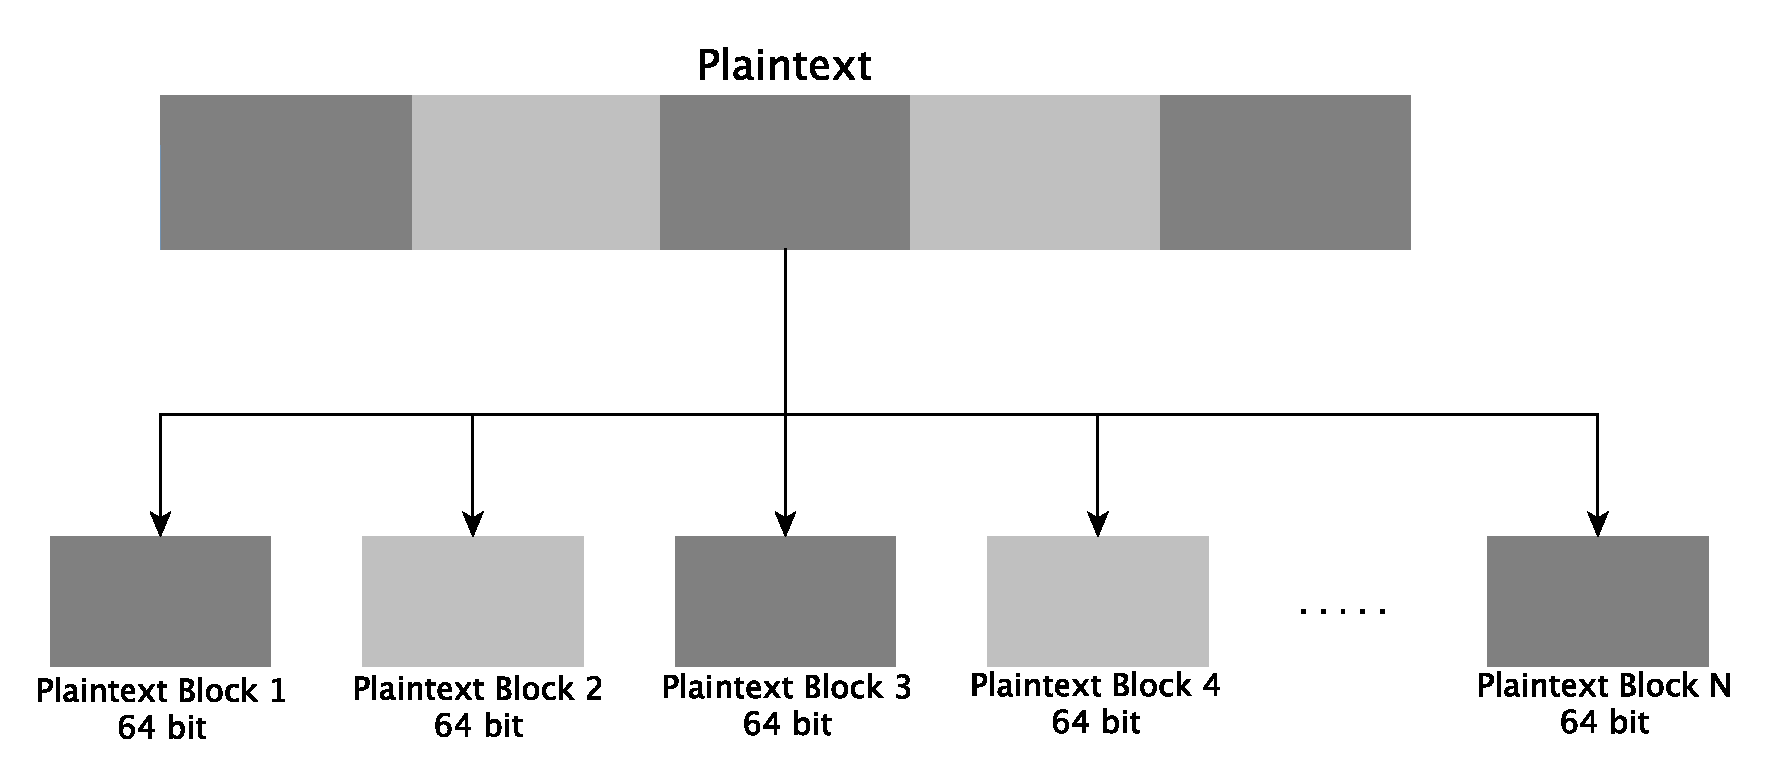
\includegraphics[scale=.37]{IMG/hashblocks}
\end{figure}
\end{frame}


\begin{frame}
\frametitle{Overview of DES}

Data is encrypted block-by-block.

\begin{figure}
\includegraphics[scale=.3]{IMG/des1}
\end{figure}

The ciphertext is constructed by combining the ciphertext blocks. 
\end{frame}


\begin{frame}[fragile]
\frametitle{DES Key}

The key for each DES block is expressed as a 64-bit number. Every eighth bit is used for parity checking and is ignored. (The parity check requires that each byte contains an odd number of \verb|1| bits.)\newline

  Thus, \textbf{the key is a 54-bit number} which can be changed at any time. 
\end{frame}



\begin{frame}
\frametitle{DES Overview}

The DES algorithm combines \textbf{confusion} and \textbf{diffusion}. \newline

DES has \textbf{16 rounds} which consist of a \textbf{substitution} followed by a \textbf{permutation}.
\end{frame}


\begin{frame}
\frametitle{DES Overview}

DES was exceptional in that it was easy to implement. It requires only standard arithmetic and logical operations. 
\end{frame}


\begin{frame}
\frametitle{DES Step 1: Initialization (Overview)}

Input: a 64-bit plaintext block.

\begin{enumerate}[(1)]
\item An initial permutation is applied to the block.
\item The block is broken into a right and a left half, each of which is 32 bits long.
\end{enumerate}

\begin{figure}
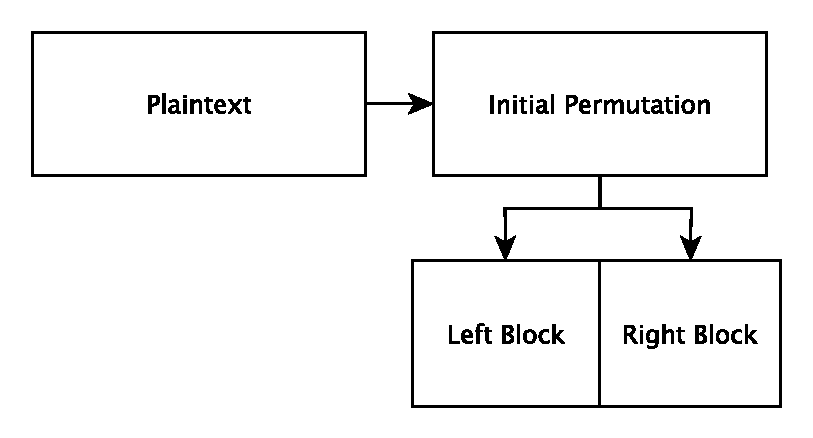
\includegraphics[scale=.5]{IMG/des3}
\end{figure}
\end{frame}


\begin{frame}
\frametitle{DES Rounds (Overview)}

Next, the DES round is carried out 16 times. 
\begin{enumerate}[(1)]
\item The key bits are \textbf{shifted}
\item
Apply the function $f$, which does the following:
\begin{itemize}
    \item 48 bits are selected from the 56 bits of the key
    \item The Right Block is expanded to 48 bits via an expansion permutation
    \item The expanded Right Block is combined with 48 bits of a shifted and permuted key via XOR
    \item This is sent through 8 \textbf{S-boxes} producing 32 new bits
    \item Permute once again.
    \end{itemize}
\item The output of $f$ is combined with the left half via XOR
\item The result is the new right half
\item The old right half becomes the new left half. 
\end{enumerate}
\end{frame}


\begin{frame}
\frametitle{DES Rounds (Overview)}
\begin{figure}
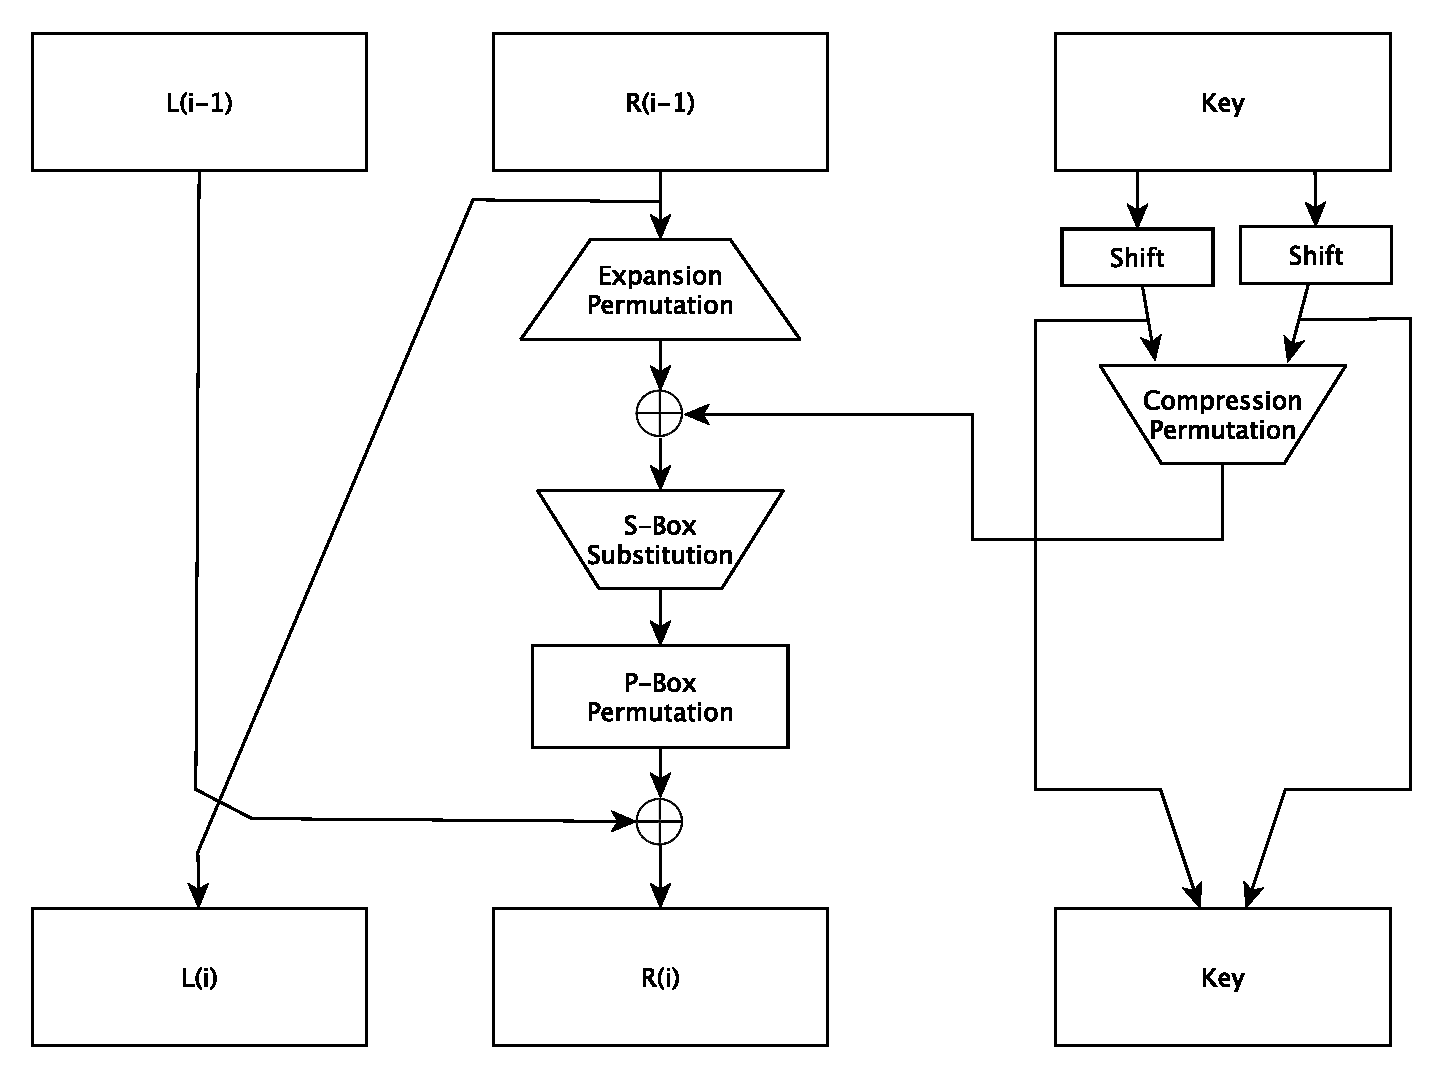
\includegraphics[scale=.4]{IMG/DESround}
\end{figure}
\end{frame}


\begin{frame}
\frametitle{Historical Note}

The initial permutation and final permutation have no affect on the security of the DES algorithm. It is postulated that the purpose of these permutations was to make it easier to load plaintexts and ciphertexts into a DES chip in byte-sized pieces, since this algoirthm predates even 16-bit microprocessor buses. 
\end{frame}

\begin{frame}
\frametitle{An Example}

Next, we will walk through the example provided in Section 12.2 of Schneier's \emph{Applied Cryptography}. See this section in the textbook for further elaboration. 
\end{frame}


\begin{frame}
\frametitle{DES Example: Initial Permutation}

Transpose the 64-bit input block according to the following table. Bit 1 of the permuted block is bit 58 of the permuted block, etc. 
\begin{figure}
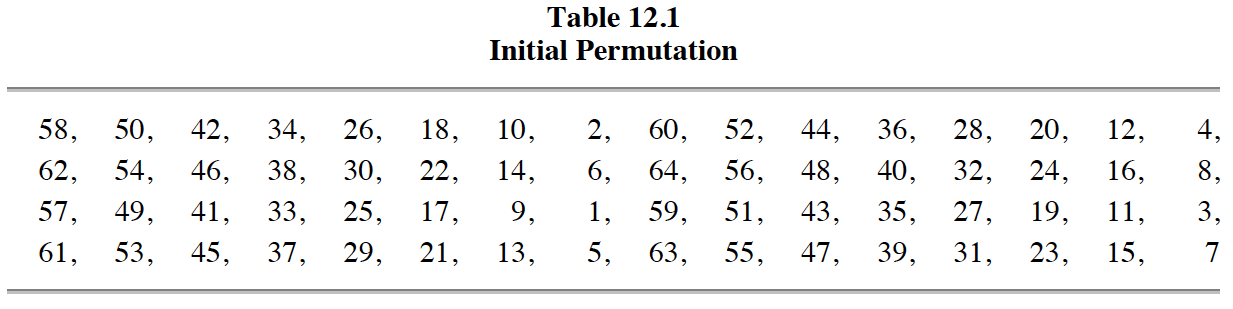
\includegraphics[scale=.5]{IMG/ex1}
\end{figure}

Because this initial permutation does not add to security, many modern applications left out the initial and final permutation steps. Though this did not affect security, it did not follow the DES standard and hence could not be called DES.
\end{frame}



\begin{frame}
\frametitle{DES Example: Key Permutation}

The 64-bit DES key is reduced to a 56-bit key by ignoring every eighth bit. This also includes the parity check.

\begin{figure}
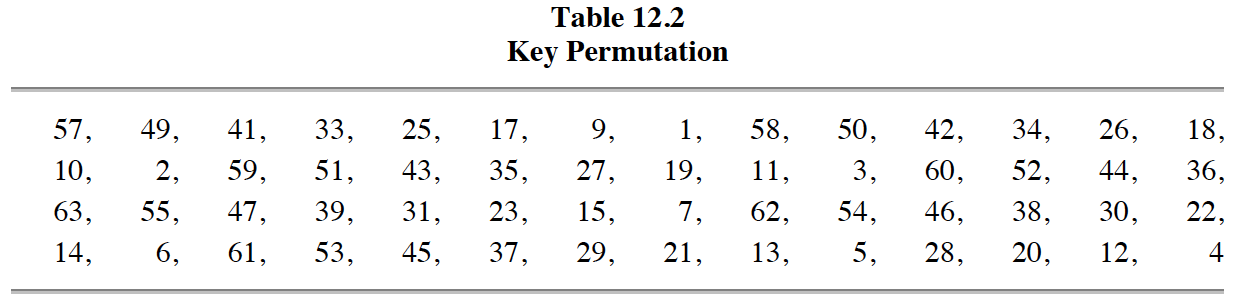
\includegraphics[scale=.5]{IMG/ex2}
\end{figure}
\end{frame}


\begin{frame}
\frametitle{DES Example: Subkeys Step 1}

A different 48-bit subkey $K_i$ is generated for each of the 16 rounds.

\begin{figure}
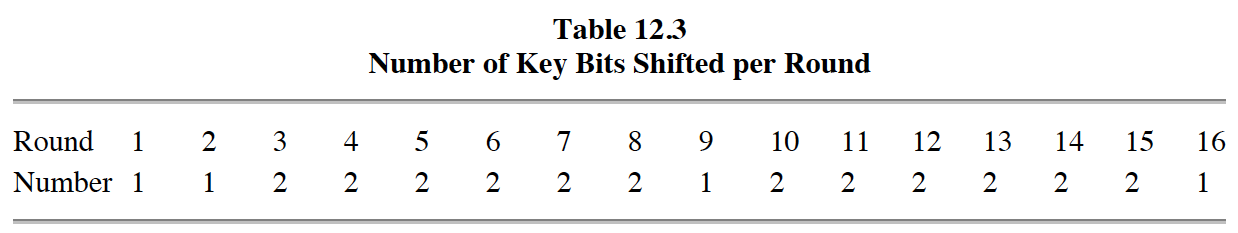
\includegraphics[scale=.5]{IMG/ex3}
\end{figure}

First, the 56-bit key is divided into two 28-bit halves. Then, the halves are circularly shifted left by
either one or two bits, depending on the round, as determined by the chart above. 
\end{frame}



\begin{frame}
\frametitle{DES Example: Subkeys Step 2}

After being shifted, 48 out of the 56 bits are selected. Because this operation permutes the order of the bits as well as selects a subset of bits, it is called a \textbf{compression permutation}. This operation provides a subset of 48 bits. 

\begin{figure}
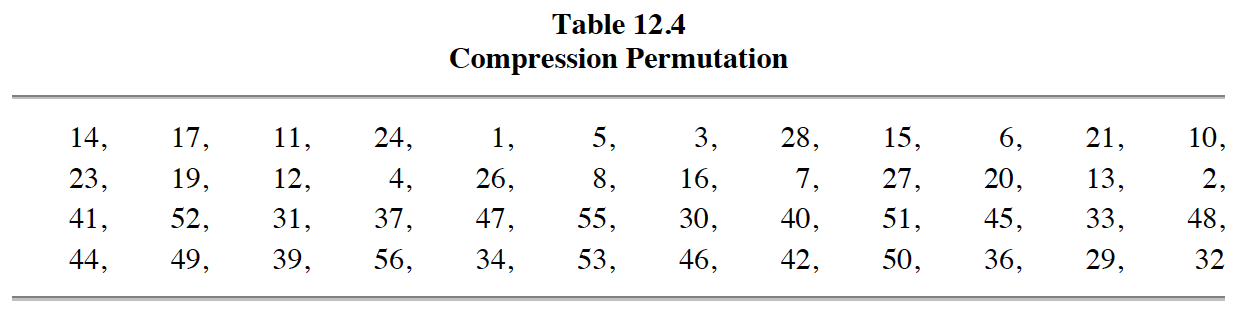
\includegraphics[scale=.5]{IMG/ex4}
\end{figure}

For example, the bit in position 14 of the shifted key moves to position 1 of the output, and the bit in position 18 of the shifted key is ignored.
\end{frame}


\begin{frame}
\frametitle{DES Example: Expansion Permutation}

The right half of the data is now expanded from 32 bits to 48 bits in what is called the \textbf{expansion permutation}. This operation makes the right half the same size as the key for the XOR operation. This expansion also provides an \textbf{avalanche effect} because it allows one bit to affect two substitutions.

\begin{figure}
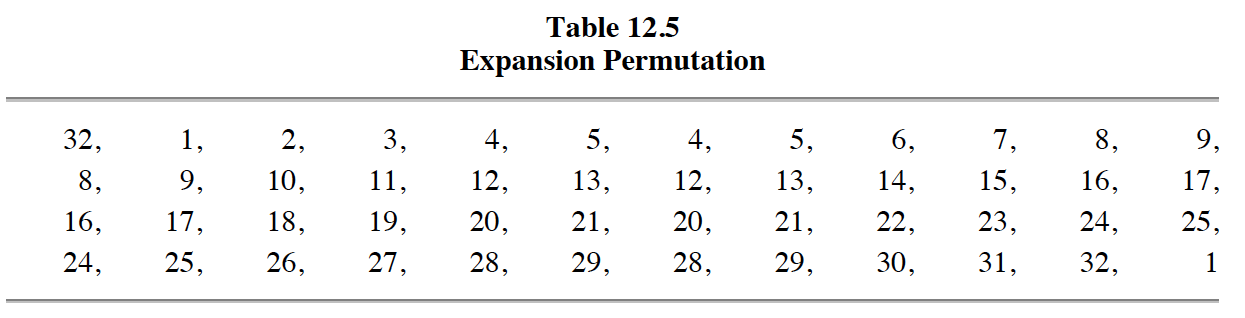
\includegraphics[scale=.5]{IMG/ex5}
\end{figure}

For example, the bit in position 3 of the input block moves to
position 4 of the output block, and the bit in position 21 of the input block moves to positions 30 and 32 of the output block.
\end{frame}



\begin{frame}
\frametitle{DES Example: Combine with XOR}

The compressed key is XOR-ed with the expanded right block.
\end{frame}


\begin{frame}
\frametitle{DES Example: S-box}

Substitutions are computed by eight \textbf{substitution boxes}, or \textbf{S-boxes}. The S-box has input of 6 bits and output of 4 bits. The 48 bits of the block are divided into eight 6-bit sub-blocks, and each sub-block is operated on by a different S-box. 

\begin{figure}
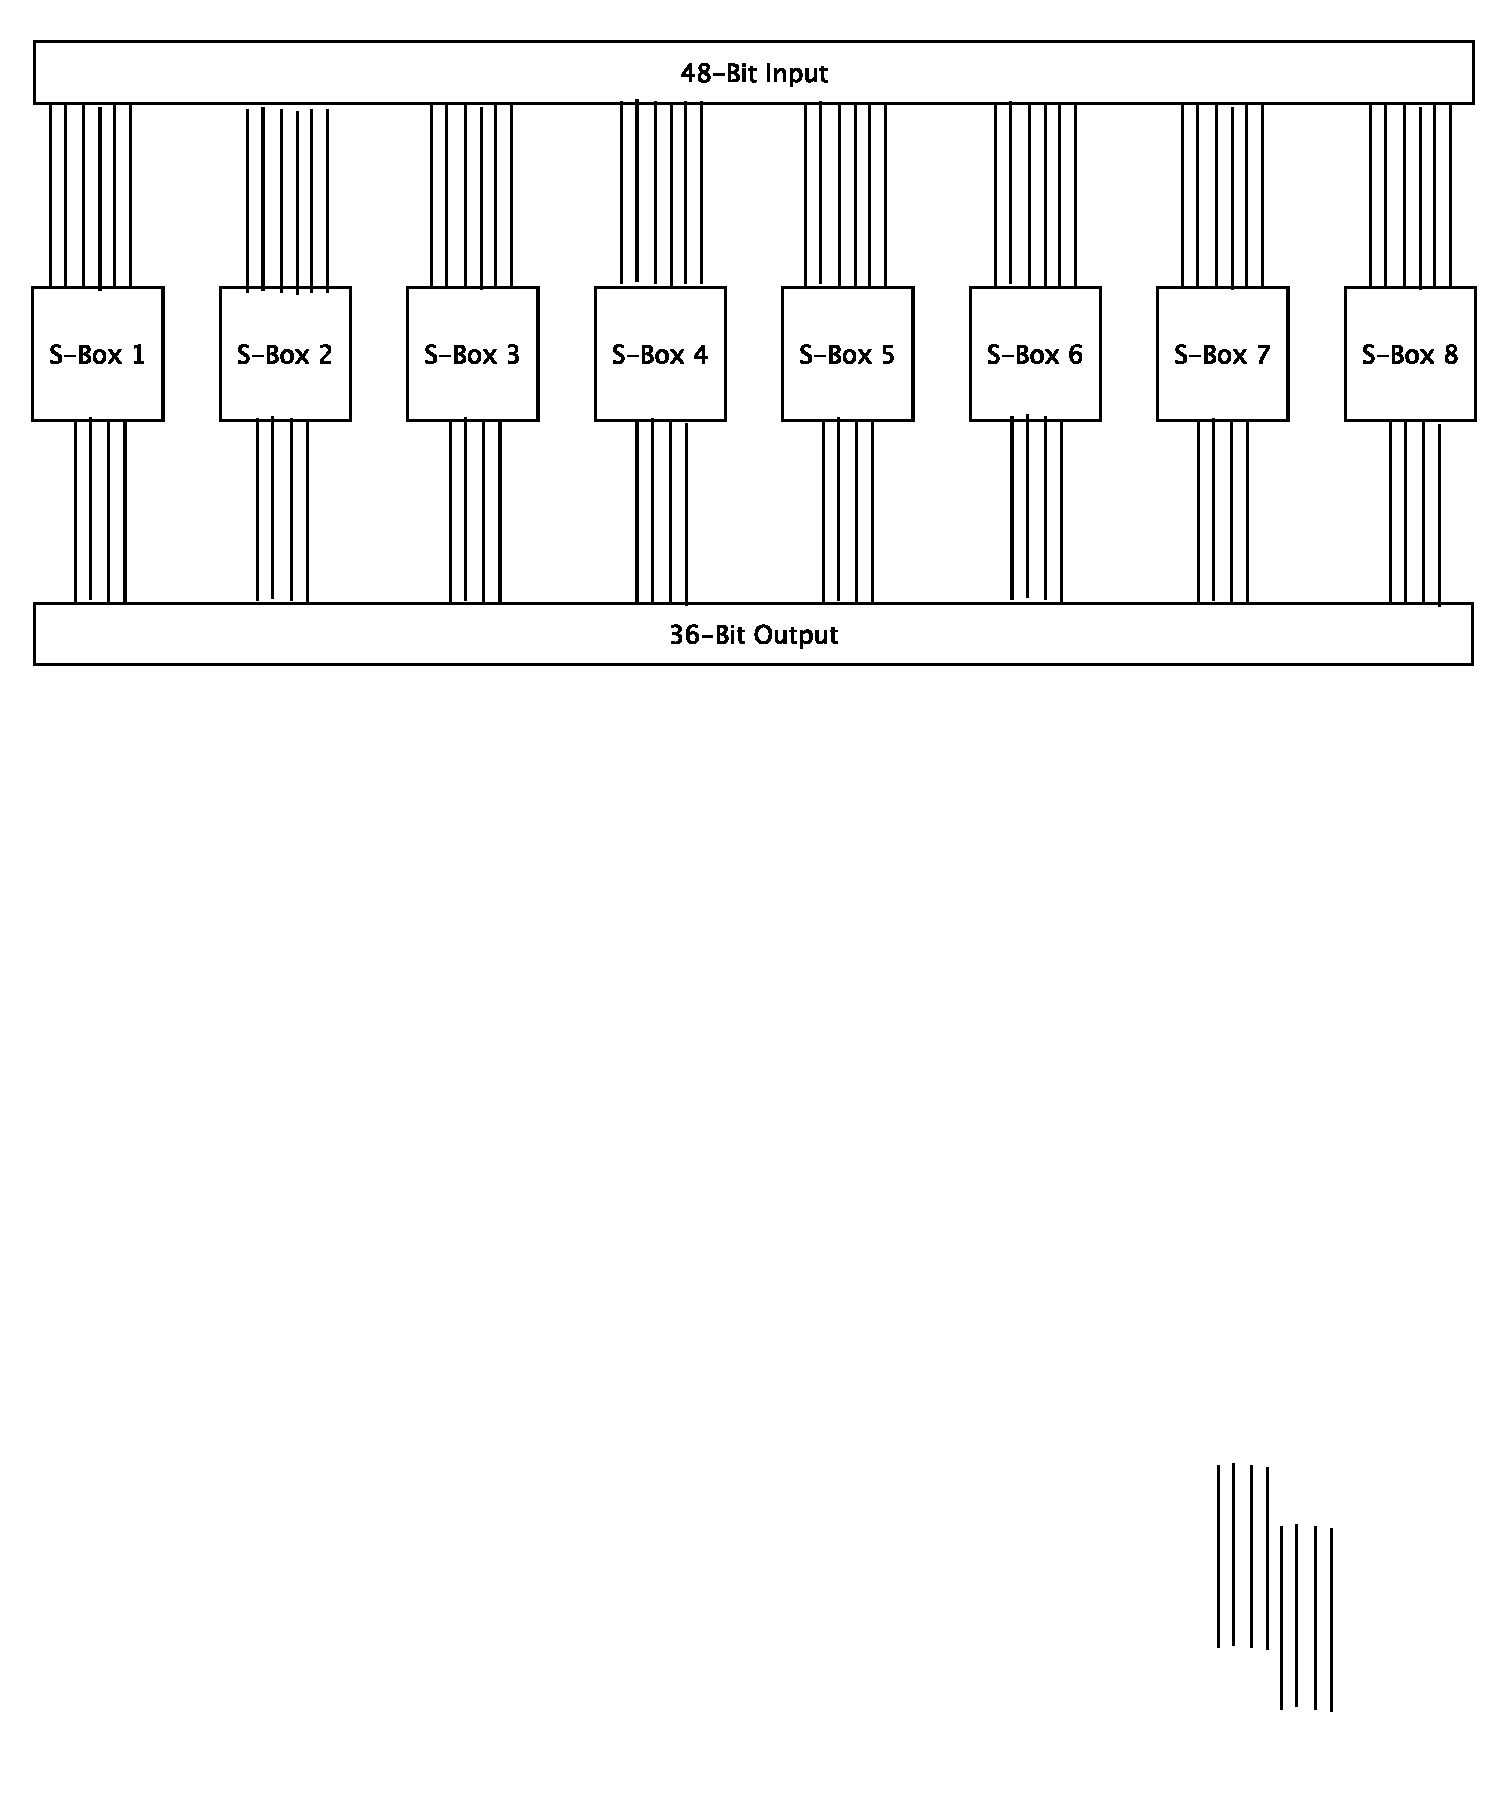
\includegraphics[scale=.45]{IMG/sbox}
\end{figure}
\end{frame}


\begin{frame}
\frametitle{DES Example: S-Box}

Each S-box is a table of 4 rows and 16 columns. Each entry in the box is a 4-bit number. The 6 input bits of the S-box specify under which row and column number to look for the output. Below are examples of what the S-boxes could look like. 

\begin{figure}
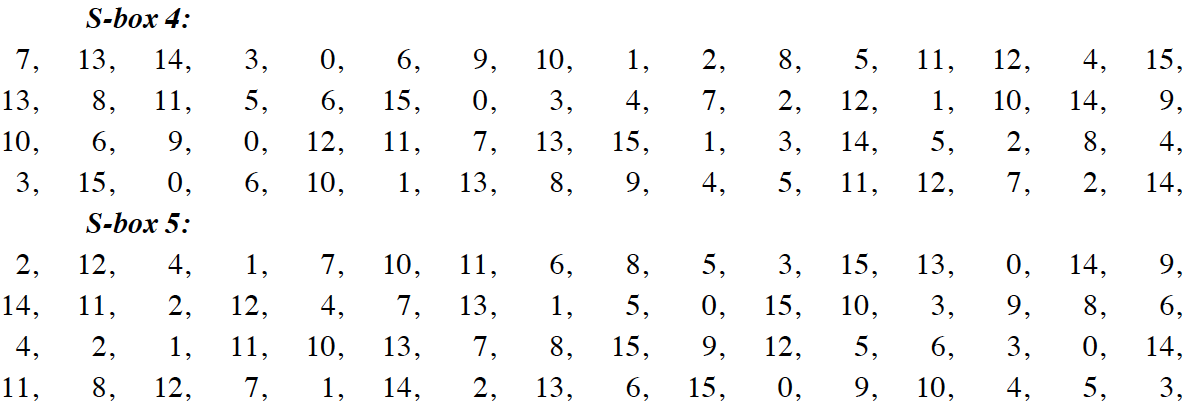
\includegraphics[scale=.5]{IMG/sbox2}
\end{figure}
\end{frame}


\begin{frame}[fragile]
\frametitle{DES Example: S-box}

Say that $b_1b_2b_3b_4b_5b_6$ is the input for an S-box. We create a 2-bit number $b_1b_6$ from 0 to 3, which corresponds to a row in the table. The middle 4 bits $b_2b_3b_4b_5$ form a 4- bit number, from 0 to 15, specifying the column.

\begin{figure}
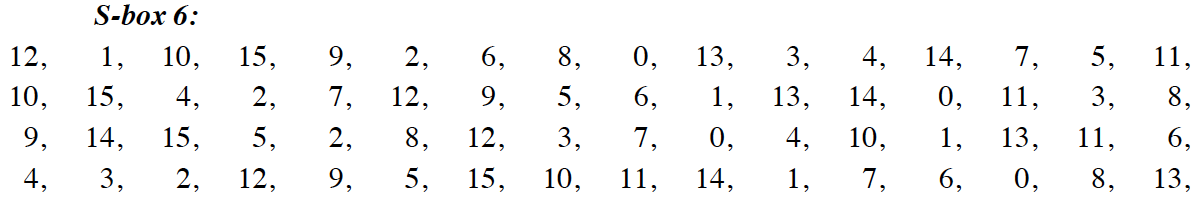
\includegraphics[scale=.5]{IMG/sbox6}
\end{figure}

Say we input \verb|110011| to S-box 6 above. The first and last bits combine to form \verb|11| (row 3). The middle 4 bits form \verb|1001| (column 9) The entry under row 3, column 9 of S-box 6 is 14. The value $14 =$ \verb|1110| is substituted for \verb|110011|.
\end{frame}


\begin{frame}
\frametitle{DES Example: S-box}

The resulting 4-bit blocks are recombined into a 32-bit block.
\end{frame}


\begin{frame}
\frametitle{DES Example: P-Box}

The 32-bit block we are left with is now permuted according to a \textbf{P-box}. 

\begin{figure}
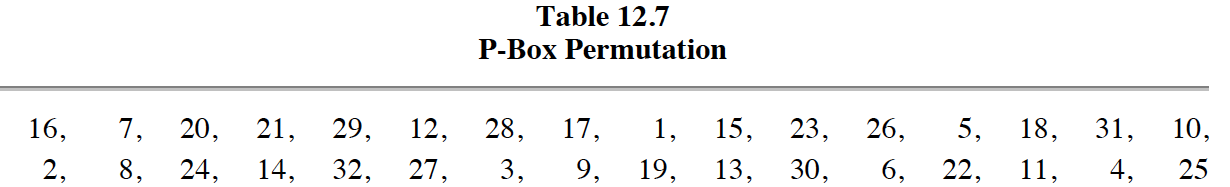
\includegraphics[scale=.5]{IMG/pbox}
\end{figure}

We XOR the result with the left half of the initial 64-bit block, then switch the left and right blocks. Another round then begins. Repeat 16 times. 
\end{frame}


\begin{frame}
\frametitle{DES Example: Final Permutation}

The final permutation is the inverse of the initial permutation. 

\begin{figure}
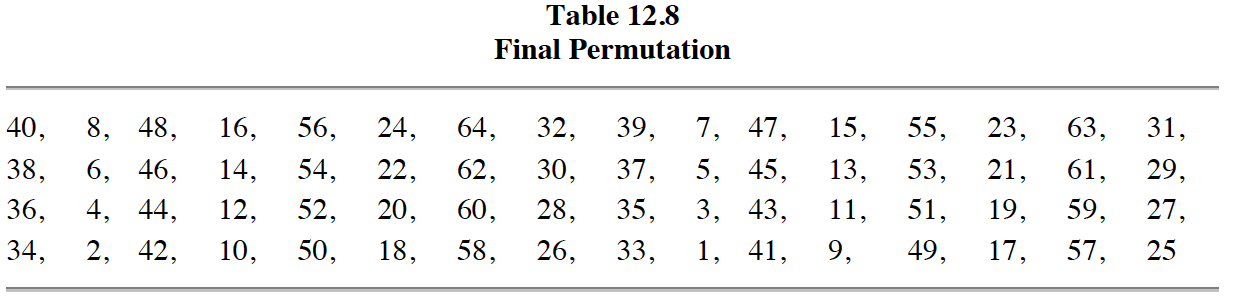
\includegraphics[scale=.5]{IMG/ex8}
\end{figure}
\end{frame}


\begin{frame}
\frametitle{DES Example: Decryption}

Decryption is the same as encryption, but the keys are used in reverse order and the key shift is a right shift. 
\end{frame}


\begin{frame}
\frametitle{References}

\begin{itemize}
\item \emph{Applied Cryptography} By Schneier, Chapter 12
\end{itemize}
\end{frame}
\end{document}


